% Projekt: IFJ15 (Interpret jazyka) - dokumentace
% Autor: Patrik Jurnečka
% Login: xjurne03
% Email: xjurne03@stud.fit.vutbr.cz
% Datum: 

\documentclass[a4paper, 11pt, titlepage]{article}
% Preambule
\usepackage[left=2cm, text={17cm, 24cm}, top=3cm]{geometry} %Rozmery
\usepackage{times} %Styl jazyka
\usepackage[IL2]{fontenc}
\usepackage[czech]{babel} %Jazyk
\usepackage[utf8]{inputenc} %Kodovani
\usepackage{graphics}
\usepackage{picture} 
\bibliographystyle{czplain}

\providecommand{\uv}[1]{\quotedblbase #1\textquotedblleft} %Uvozovky 

\begin{document} %Textova cast

\begin{titlepage} %Titulni strana
\begin{center}
\textsc{\Huge{Vysoké učení technické v~Brně}\\[3mm]\huge{Fakulta informačních technologií}}\\

\vspace{\stretch{0.1}}

\begin{figure}[h]
	\centering
	\scalebox{0.17}{\includegraphics{FIT_zakladni_provedeni_loga.jpg}}
\end{figure}

\vspace{\stretch{0.042}}
\huge{Dokumentace projektu do předmětu IFJ a IAL}\\
\Huge{\textbf{Interpret jazyka IFJ15}}\\
\LARGE{Tým 043, varianta b/2/I}
\vspace{\stretch{0.618}}
\end{center}

{\noindent\Large \hfill Martin Honza (xhonza03)\\}
{\indent\Large \hfill Patrik Jurnečka (xjurne03)\\}
{\indent\Large \hfill Hana Slámová (xslamo00)\\}
{\indent\Large \hfill Frantisek Šumšal (xsumsa01)\\}
{\indent\Large\today \hfill Adam Švidroň (xsvidr00)}

\end{titlepage}

\tableofcontents

\newpage

\section{Úvod} %Uvod
Dokumentace popisuje návrh a implementaci projektu Interpret jazyka IFJ15 do předmětu IFJ (Formální jazyky a~překladače) a IAL (Algoritmy). Vybrali jsme si zadání b/2/I, které nám udávalo, jáký algoritmus máme pro daný problém využít. Pro vyhledávání \textbf{Boyer-Mooreův algoritmus}, pro řazení algoritmus Heap sort, který byl využit ve vestavěné funkci \textbf{sort}. Poslední ze specifikových pravidel použití, jsme měli využít k implementaci tabulky symbolů \textbf{binární vyhledávací strom}. 

Cílem projektu bylo vytvořit program, který interpretuje jazyk IFJ15, což je velmi zjednodušenou podmnožinou jazyka C++11. 

\section{Struktura projektu}
Překladač je rozdělen do tří hlavních celků. Pomocí \textbf{lexikálního analyzátoru} načítá zdrojový kód. \textbf{Syntaktický analyzátor} zažádá lexikální o token a ověří syntaxi a sémantiku. Po bezchybné kontrole se spustí \textbf{interpret}.  

\section{Lexikální analizátor (scanner)}
Analyzátor je implementován v souborech \textit{lex.c} a \textit{lex.h}. Lexikální analyzátor načítá zdrojový kód po znacích a převádí jej na tokeny. Veškerá komunikace s dalšími knihovnami probíhá pomocí funkce \textit{lex\_get\_token}. Analyzátor je Implementován pomocí konečného automatu (Obrázek~\ref{picture_1:konecny_automat}), přičemž veškeré komentáře ignoruje. Funkce je volána vždy, když syntaktický analyzátor zažádá o~token. 

Token definuje jednotlivé prvky kódu a určuje jak se k němu má při překladu přistupovat. Analyzátor prochází tabulku klíčových slov (\textit{lex\_kw\_t keywords[]}), zda-li nejde o rezervované klíčové slovo pro speciální funkci.

\subsection{Konečný automat}

\begin{figure}[h]
	\centering
	\scalebox{0.15}{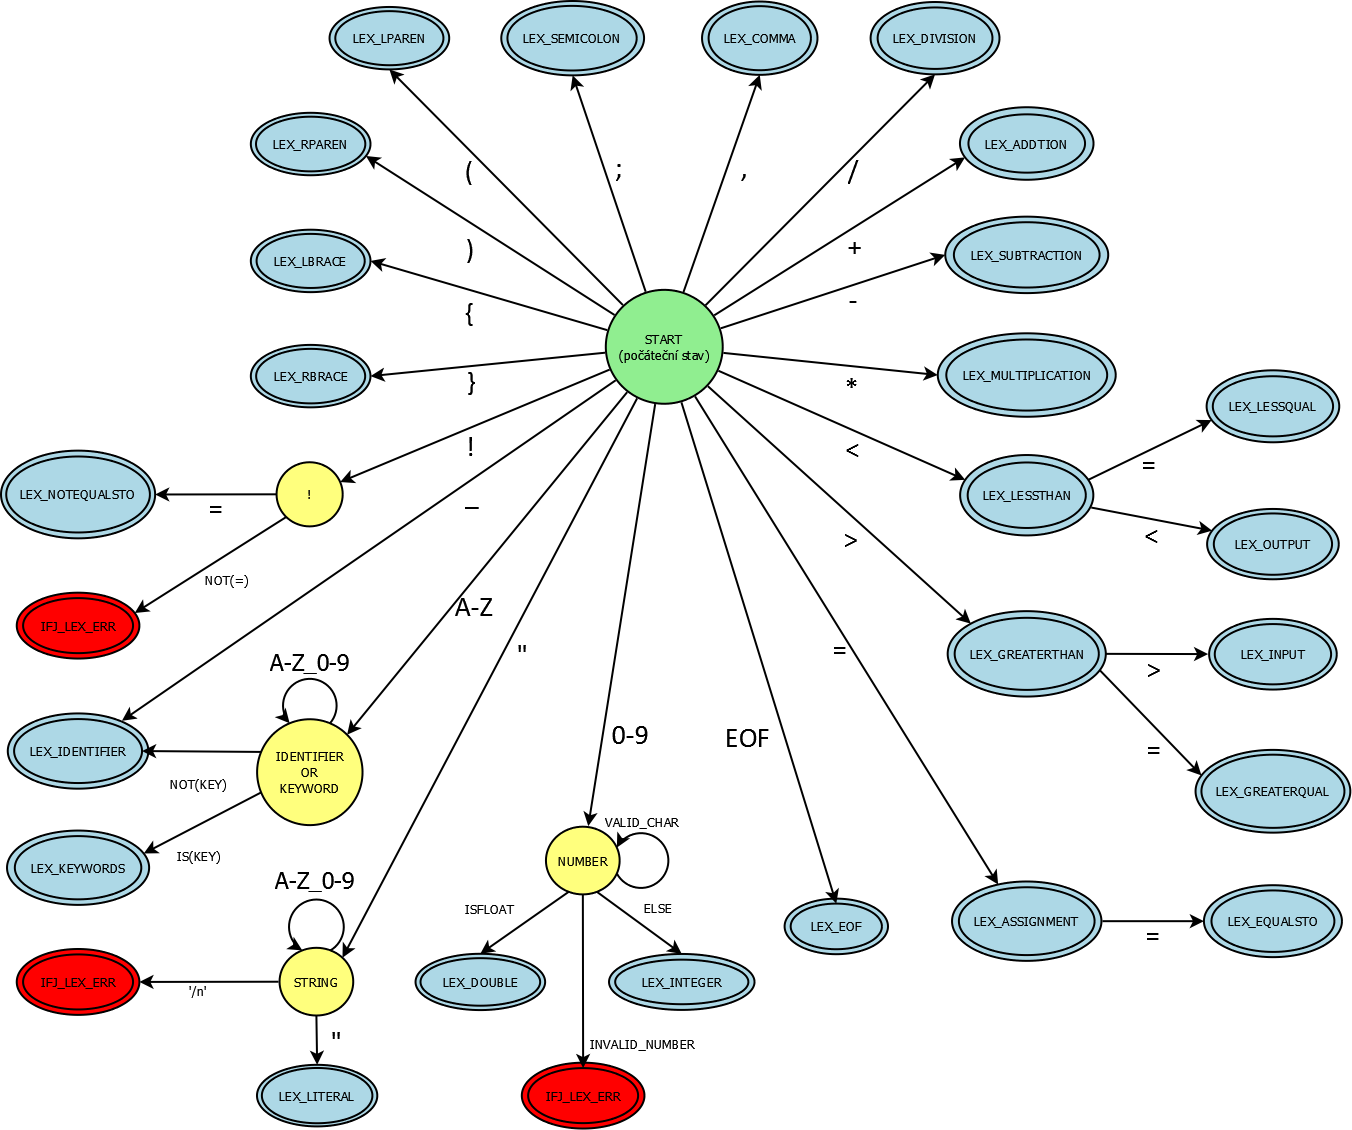
\includegraphics{konecny_automat.png}}
	\caption{Konečný automat}
	\label{picture_1:konecny_automat}
\end{figure}

\newpage
\section{Syntaktická analizátor (parser)}
Syntaktický analyzátor postupně volá tokeny z lexikálního analyzátoru. Tokeny jsou zpracovávaný dvěma způsoby. Pomocí LL gramatiky (Tabulka \ref{table_1:LL_gramatic}) a precedenční syntaktické analýzy (Tabulka \ref{table_2:PA}). Při úspěšném dokončení syntaktické analýzy se generuje instrukční páska pro interpret.

\subsection{LL gramatika}
LL gramatika postupně ověřuje příchozí tokeny.   

\begin{table}[h]
\footnotesize
	\begin{center}
	\begin{tabular}{c c l}
	1.  & $<program>$ 	 & 	$<declrList>$ EOF \\ 
	2.  & $<declrList>$  &  $<funcDeclr>$ $<declrList>$ \\ 
	3.  & $<declrList>$  &  $<empty>$ \\ 
	4.  & $<funcDeclr>$  &  $<typeSpec>$ ID ($<params>$) \\
	5.  & $<typeSpec>$ 	 &  INT \\
	6.  & $<typeSpec>$   &  DOUBLE \\ 
	7.  & $<typeSpec>$ 	 &  STRING \\ 
	8.  & $<params>$ 	 & 	$<paramItem>$ \\ 
	9.  & $<params>$ 	 & 	$<paramItem>$, $<params>$ \\ 
	10. & $<paramItem>$  & 	$<typeSpec>$ ID\\ 
	11. & $<paramItem>$  & 	$<empty>$ \\ 
	\end{tabular}
	\caption{LL gramatika}
	\label{table_1:LL_gramatic}
	\end{center}
\end{table}

\subsection{Precedenční syntaktická analýza}
Syntaktická analýza zdola nahoru. Dle Zadání jsem analýzu implementovali za pomocí precedenční tabulky, která nám pomáhá ošetřit vstupní výrazy.

\begin{table}[h]
	\begin{center}
	\begin{tabular}{l | c c c c c c c c c c c c c c}
			  & $+$ & $-$ & $*$ & $/$ & $<$ & $>$ & $<=$& $>=$& $==$ & !$=$ &  $($   &  $)$   &  id  &    \$ \\ \hline
		$+$   & $>$ & $>$ & $<$ & $<$ & $>$ & $>$ & $>$ & $>$ & $>$  & $>$  & $<$  & $>$  & $<$  & $>$ \\
		$-$   & $>$ & $>$ & $<$ & $<$ & $>$ & $>$ & $>$ & $>$ & $>$  & $>$  & $<$  & $>$  & $<$  & $>$ \\
		$*$   & $>$ & $>$ & $>$ & $>$ & $>$ & $>$ & $>$ & $>$ & $>$  & $>$  & $<$  & $>$  & $<$  & $>$ \\
		$/$   & $>$ & $>$ & $>$ & $>$ & $>$ & $>$ & $>$ & $>$ & $>$  & $>$  & $<$  & $>$  & $<$  & $>$ \\
		$<$   & $<$ & $<$ & $<$ & $<$ & $<$ & $>$ & $>$ & $>$ & $>$  & $>$  & $<$  & $>$  & $<$  & $>$ \\
		$>$   & $<$ & $<$ & $<$ & $<$ & $<$ & $>$ & $>$ & $>$ & $>$  & $>$  & $<$  & $>$  & $<$  & $>$ \\
		$<=$  & $<$ & $<$ & $<$ & $<$ & $<$ & $>$ & $>$ & $>$ & $>$  & $>$  & $<$  & $>$  & $<$  & $>$ \\
		$>=$  & $<$ & $<$ & $<$ & $<$ & $<$ & $>$ & $>$ & $>$ & $>$  & $>$  & $<$  & $>$  & $<$  & $>$ \\
		$==$  & $<$ & $<$ & $<$ & $<$ & $<$ & $>$ & $>$ & $>$ & $>$  & $>$  & $<$  & $>$  & $<$  & $>$ \\
		!$=$  & $<$ & $<$ & $<$ & $<$ & $>$ & $>$ & $>$ & $>$ & $>$  & $>$  & $<$  & $>$  & $<$  & $>$ \\
		$($   & $<$ & $<$ & $<$ & $<$ & $<$ & $<$ & $<$ & $<$ & $<$  & $<$  & $<$  & $=$  & $<$  &     \\
		$)$   & $>$ & $>$ & $>$ & $>$ & $>$ & $>$ & $>$ & $>$ & $>$  & $>$  &      & $>$  &      & $>$ \\
		id    & $>$ & $>$ & $>$ & $>$ & $>$ & $>$ & $>$ & $>$ & $>$  & $>$  &      & $>$  &      & $>$ \\
		\$    & $<$ & $<$ & $<$ & $<$ & $<$ & $<$ & $<$ & $<$ & $<$  & $<$  & $<$  &      & $<$  &     \\ \hline
	\end{tabular}
	\caption{Precenenční tabulka syntaktické analýzy výrazů}
	\label{table_2:PA}
	\end{center}
\end{table}

\newpage

\section{Sémantický analizátor}

\section{Interpret}
Poslední částí Interpretu je vlastní překlad, který nastane pouze pokud zdrojový kód úspěšně projde syntaktickou a sémantickou analýzou. Interpretační část ma za úkol zpracovat instrukční sadu založenou na 3AC (tří adresné instrukce).

\section{Chybové stavy}
Pro chybové stavy jsme implementovali vlastní funkci, která je vždy volána při nalezení chyby v kód, jak syntaktické, sémantické nebo při interpretaci. Návratové chybové kódy byly definovány v zadání projektu. 

\newpage

\section{Algoritmy z předmětu IAL}

\subsection{Heapsort}
Heapsort neboli \uv{řazení hromadou} je řadící metoda s lineární složitostí. Algoritmus patří mezi nestabilní algoritmy, protože přesouvá prvky s příliš velkými skoky a také se nechová přirozeně.  

\subsection{Boyer-Mooreův algoritmus}
Dle zadání jsem měli vestavěnou funkci \textbf{find}, která by používala pro vyhledání Boyer-Mooreův algoritmus.
Boyer-Mooreův algoritmus je jedním velmi efektivním algoritmem pro vyhledávání podřetězců v řetězcích. Algoritmus prochází textem a porovnává vzorek zprava doleva a pro posuv bere ten z výsledků dvou heuristik,
který je výhodnější. Jeho efektivita spočívá v časové složitosti. Čím delší je vyhledávaný podřetězec, tím je kratší doba. Funkce je implementována podle skript z předmětu IAL.

\begin{itemize}
	\item ComputerJumps()
	\subitem Stanovení hodnot pole \textit{CharJump}, které určují posuv vzorku. Použití pole CharJump pro postup vzorku činí tento algoritmus mnohem rychlejší než algoritmus Knuth-Morris-Prattův. 
	
	\subitem Jednotlivé symboly řetězce mají uloženou svojí ASCII hodnotu. 
	
	\item ComputerMatchJumps()
	\subitem Funkce pro samotný výpočet pole \textit{MatchJump}.
	
	\item Boyer\_Moor\_Alg()
	\subitem Stanovení indexu polohy vzorku nalezeného v textu.
	
\end{itemize}

\subsection{Binární vyhledávací strom (BVS)}
Nejpoužívanější implementace pro dynamické vyhledávací tabulky. Algoritmus je implementován rekurzivně, dle opory k předmětu IAL (algoritmy). Vyhledávání v BVS je velmi podobné binárnímu vyhledávání v seřazeném poli.  

Vytvořili jsme vlastní knihovnu funkcí. Implementace knihovny je v souborech \textit{bst.c} a \textit{bst.h}. 

Rozhraní bst poskytuje funkčnost specifickou pro tabulku symbolů, která je implementována v souborech \textit{stable.c} a \textit{stable.h}.

\newpage

\section{Práce v týmu}
Komunikace v týmu probíhala za pomocí IRC Freenode. Pravidelná osobní setkání se uskutečňovalo jednou za čtrnáct dní nebo po domluvě v CVT. Na osobním setkání bylo objasněno, co vše je zapotřebí udělat a také provedeno rovnoměrné rozdělení práce.

Ke sdílení zdrojových kódů jsme využili GitHub s vlastním soukromým kanálem. 

\subsection{Rozdělení práce}

\begin{itemize}
	\item\textbf{Martin Honza:} Precedenční analýza výrazu
	\item\textbf{Patrik Jurnečka:} Dokumentace, prezentace
	\item\textbf{Hana Slámová:} Vestavěné funkce
	\item\textbf{Frantisek Šumšal:} Lexikální analýzátor, syntaktický analyzátor
	\item\textbf{Adam Švidroň:} Heap sort, interpret
\end{itemize}  

\section{Závěr}
Na projektu se pracovalo téměř dva měsíce, i když jsme začali včas, dokončit projekt jsme nestíhali do pokusného odevzdání. V posledním týdnu před odevzdáním jsme dodělávali interpret a snažili se vše zkompletovat, aby fungoval projekt dle zadání. Dokumentace se tvořila průběžně při dokončení některého logického celku. 

Projekt byl velmi náročný, nejen ze strany programové, ale také hlavní roli hrála domluva týmu. Nakonec se to zvládlo dokončit. Z projektu jsme si odnesli velké zkušenosti, jak efektivně organizovat a pracovat v týmu.

Navržená implementace byla nakonec otestována v prostředí operačních systémů Linux a MS Windows 10.

Dokumentace i prezentace jsme psali v jazyce \LaTeX. 

\subsection{Metriky kódu}
\begin{itemize}
	\item Počet souborů: ...
	\item Počet řádků zdrojového kódu: ...
	\item Velikost spustitelného souboru: ... (OS Linux 32 bitová architektůra)
\end{itemize}  

\nocite{Ahoc2007}
\bibliography{literatura}

\end{document} %konec textove casti